\section{Model Analysis}

\begin{frame}{Linearization and Transfer function $G(s)$}

    Considering linearization around the position of $10 [mm]$, the following state-space representation of the system is obtained:

    \begin{equation}
        A =
        \begin{bmatrix}
            0    & 1 & 0      \\
            1555 & 0 & -20.63 \\
            0    & 0 & -35.55
        \end{bmatrix}
        \quad
        B =
        \begin{bmatrix}
            0 \\
            0 \\
            99.41
        \end{bmatrix}
    \end{equation}

    \begin{equation}
        C =
        \begin{bmatrix}
            1 & 0 & 0
        \end{bmatrix}
        \quad
        D =
        \begin{bmatrix}
            0
        \end{bmatrix}
    \end{equation}

    Based on this, the transfer function $G(s)$ of the system is given by:

    \begin{equation}
        G(s) = C \left( sI - A \right)^{-1} B + D = \frac{-2051}{s^3 + 35.56 s^2 - 1555 s - 5.53\cdot10^4}
    \end{equation}

\end{frame}



\begin{frame}{Stability analysis}

    \begin{columns}[c, onlytextwidth]

        \begin{column}{0.60\textwidth}

            \begin{figure}[H]
                \centering
                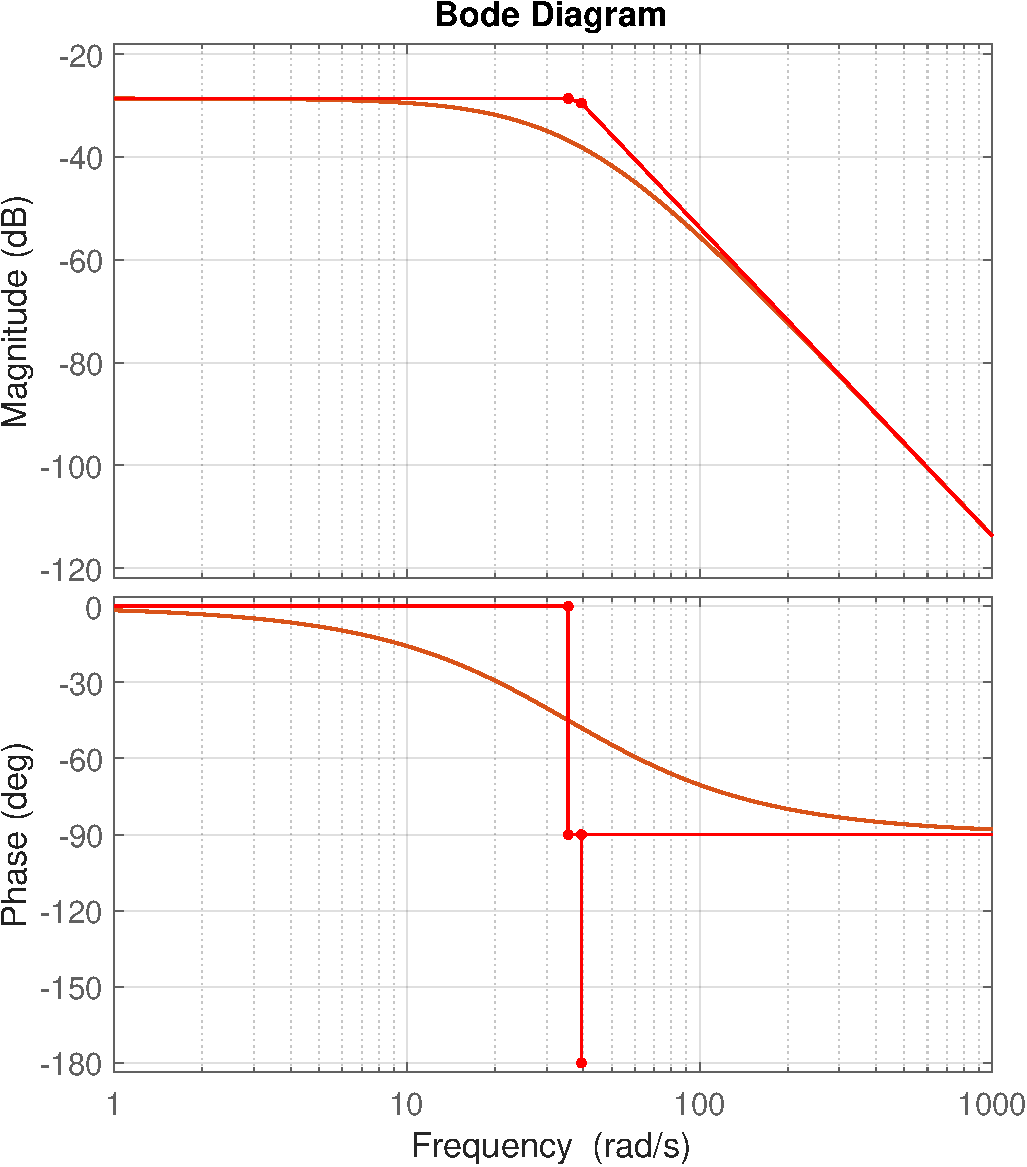
\includegraphics[width=0.8\textwidth]{./img/MATLAB/analysis/bode_plot_resized.pdf}
                \caption{Bode plot for the transfer function $G(s)$.}
            \end{figure}

        \end{column}

        \begin{column}{0.40\textwidth}

            The Bode plot shows that the system is unstable, as the gain margin is negative.

            \vspace{9pt}

            Instability is also confirmed by the poles of the system:

            \begin{equation}
                eig(A) =
                \begin{cases}
                    39.44  \\
                    -39.44 \\
                    -35.56
                \end{cases}
            \end{equation}

        \end{column}

    \end{columns}

\end{frame}



\begin{frame}{Stability analysis}

    \begin{figure}[H]
        \centering
        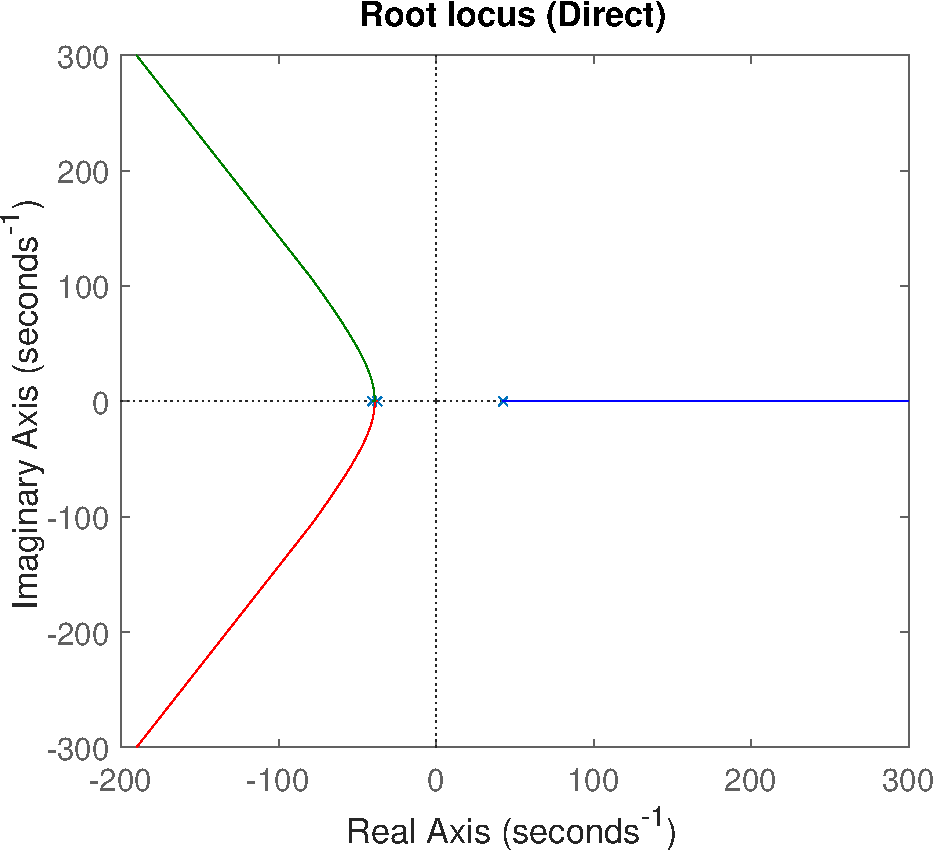
\includegraphics[width=0.47\textwidth]{./img/MATLAB/analysis/root_locus_direct.pdf}
        \hfill
        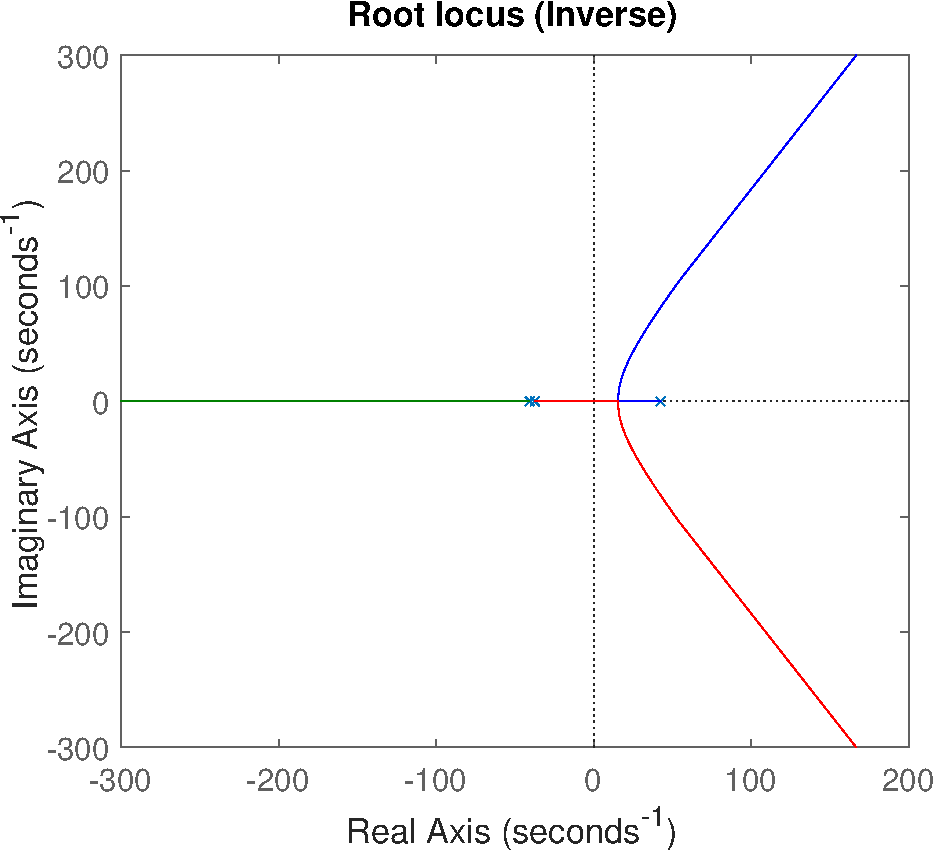
\includegraphics[width=0.47\textwidth]{./img/MATLAB/analysis/root_locus_inverse.pdf}
        \caption{Root Locus plot with positive and negative proportional feedback control.}
        \label{fig:root_locus_plot}
    \end{figure}


\end{frame}



\begin{frame}{Controllability and reachability}

    Luckily, the system is controllable and reachable, as the rank of both the controllability and reachability matrices is equal to the number of states.

    \vspace{9pt}

    We can now move on to the design of estimators and controllers for the system.

\end{frame}